\documentclass{beamer}
\usepackage[latin1]{inputenc}
\usepackage{amsmath}
\usepackage{graphicx}
\usepackage{multimedia}
\usetheme{default}
\usecolortheme{default}
\definecolor{darkred}{RGB}{24,0,0}
\setbeamercolor{title}{fg=red}
\setbeamertemplate{blocks}[rounded][shadow=true]
\setbeamertemplate{itemize items}[square]
\usefonttheme{serif}
\title[Make a LaTeX presentation using Beamer]{The effect of gas bulk 
rotation in the morphology of the Ly$\alpha$ line.}
\author{Juan Nicol\'as Garavito-Camargo \\ Advisor: Jaime E. Forero-Romero}
\institute{Universidad de los Andes, Bogot\'a, Colombia}
\date{May 20, 2015}
\begin{document}

\begin{frame}
\titlepage
\author
\institute
\begin{figure}
%\rule{1.28cm}{0.72cm}

\includegraphics[scale=0.35]{Figures/logo.jpeg}
\end{figure}
\end{frame}


\begin{frame}{Lyman $\alpha$ emission line:}
A Ly$\alpha$ photon is emitted with a $\lambda= 121.56 nm$.
\begin{figure}
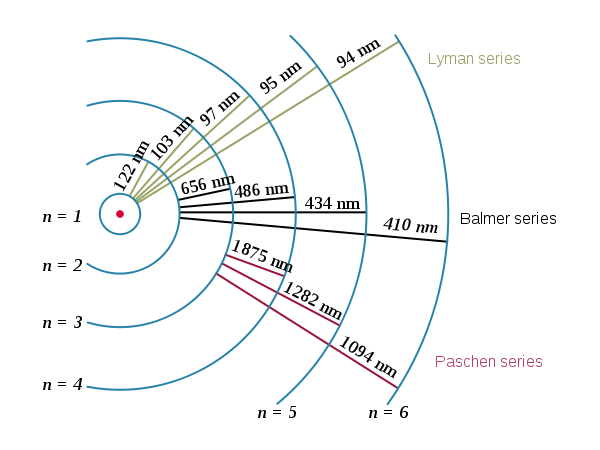
\includegraphics[scale=0.4]{Figures/Hydrogen_transitions.png}
\end{figure}
\end{frame}

\begin{frame}{Ly$\alpha$ is in the vacuum UV part of the EM spectrum}
\begin{figure}
\centering
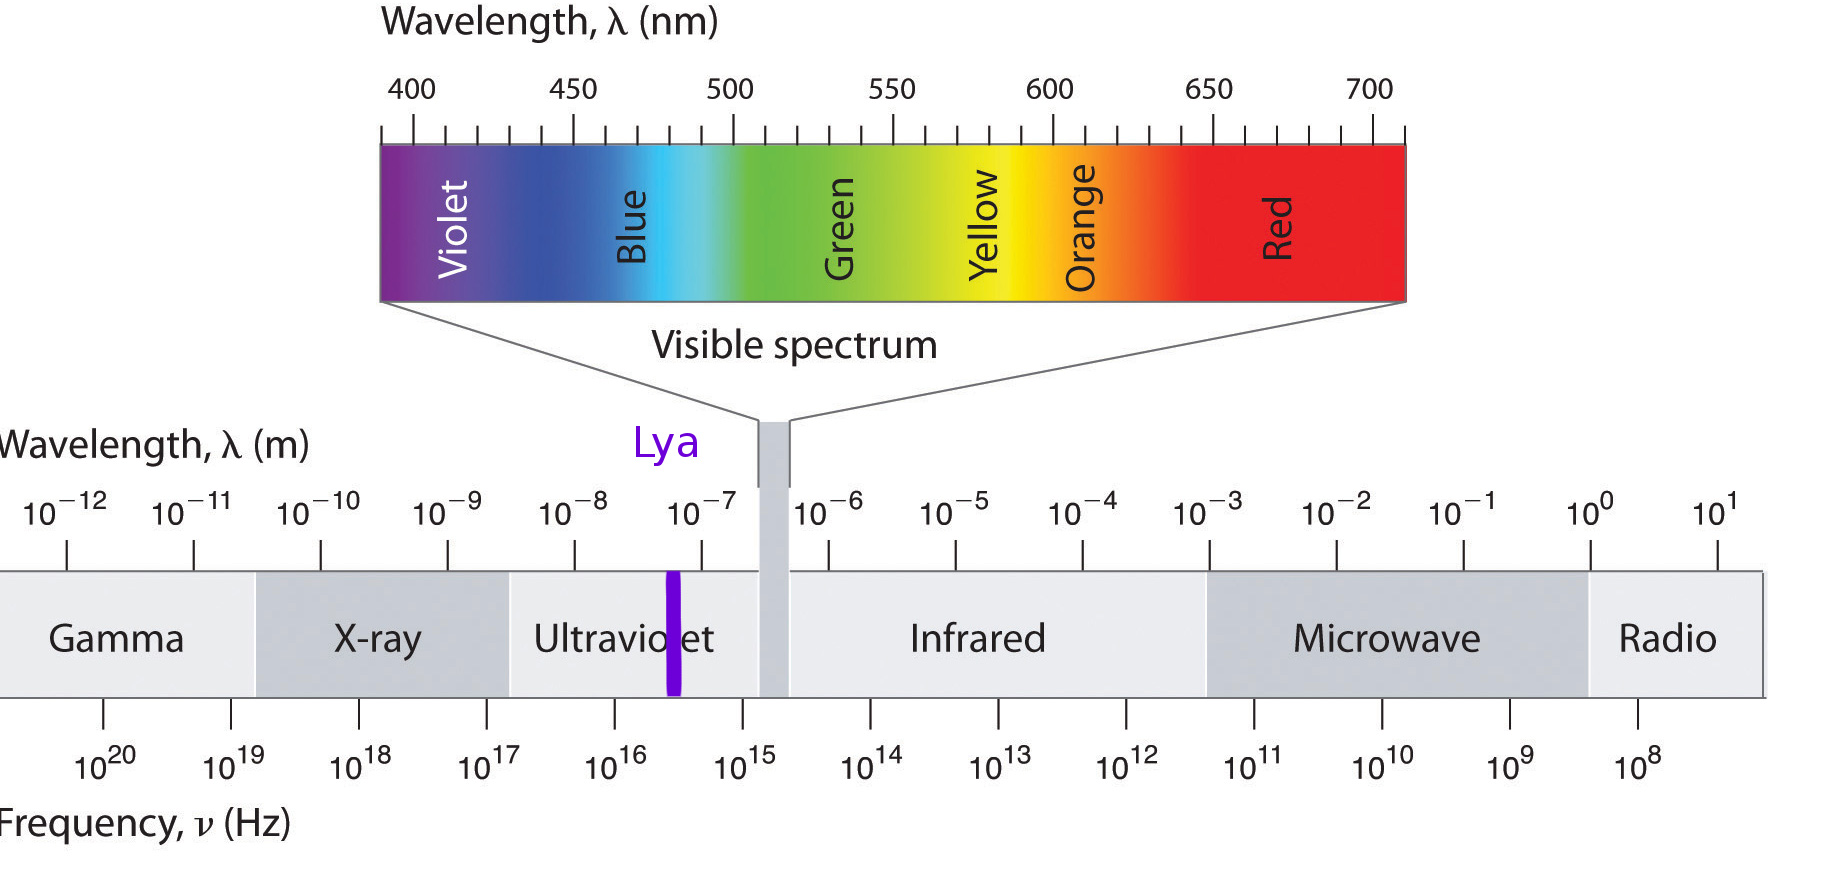
\includegraphics[scale=0.18]{Figures/em.jpg}
\end{figure}
\end{frame}


\begin{frame}
\begin{figure}
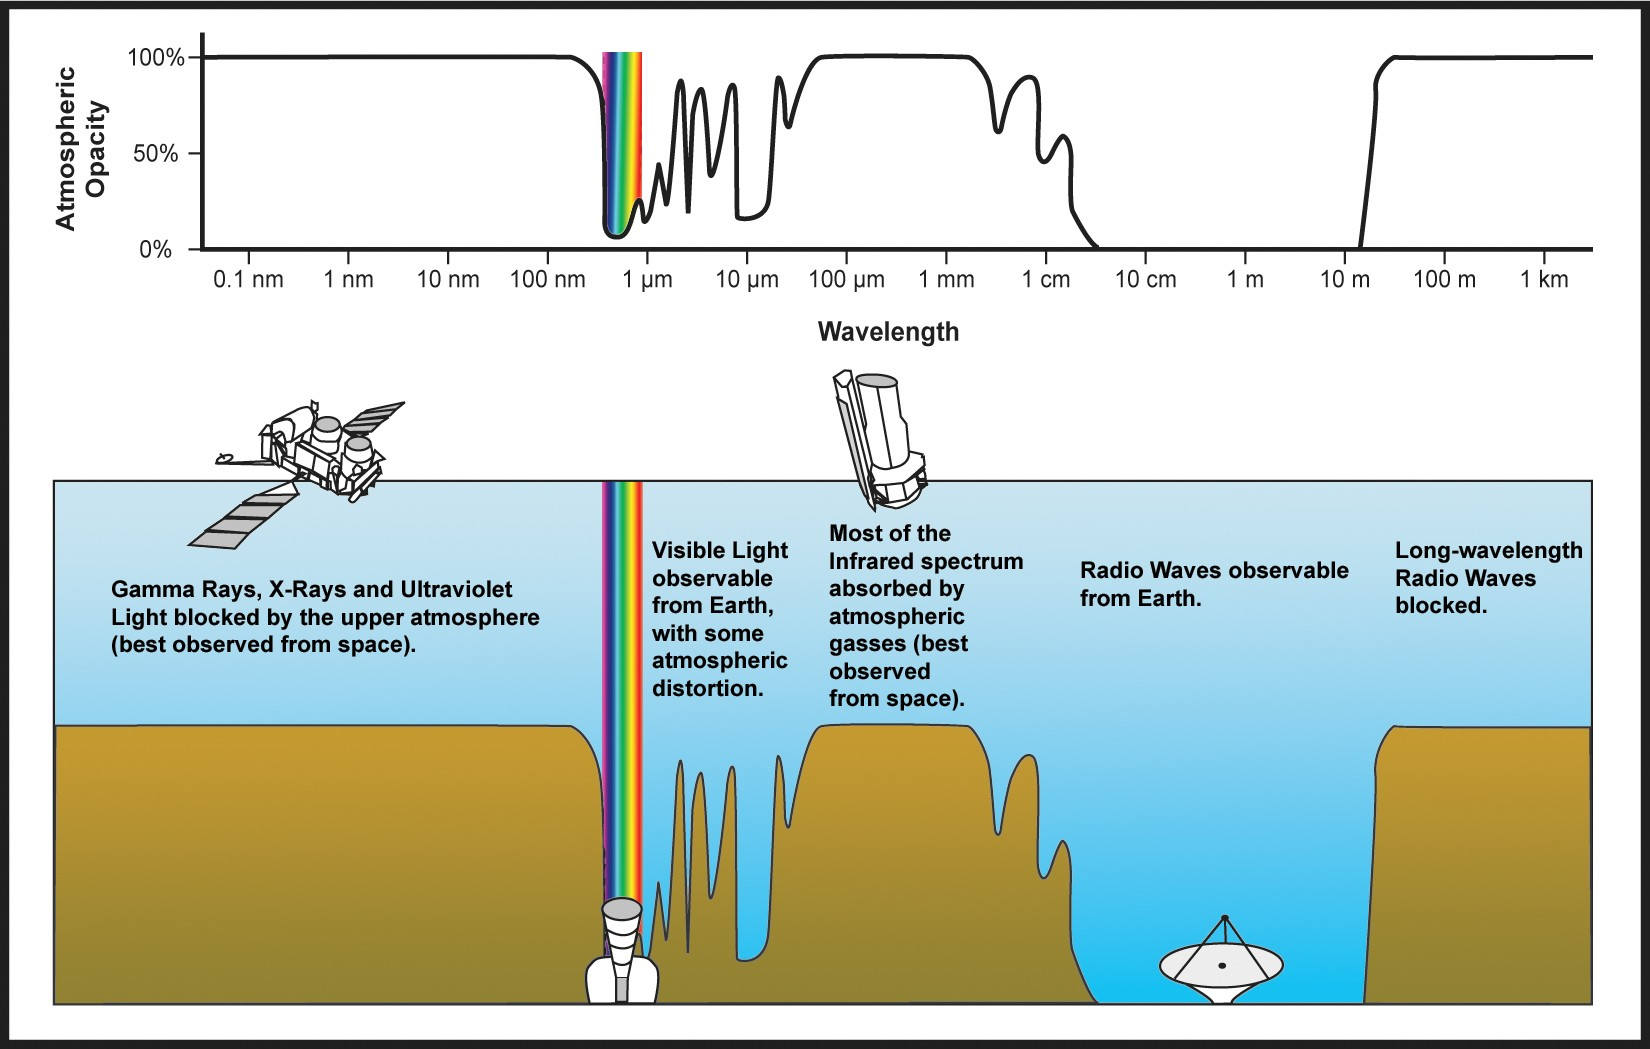
\includegraphics[scale=0.8]{Figures/AtmosphericEM.jpg}
\caption{Atmospheric radiation absorption}
\end{figure}
\end{frame}


%\begin{frame}
%Lya line characteristics
%\end{frame}

\begin{frame}{Cosmological Redshift \& the observable LAEs in the visible regime.}
\begin{figure}
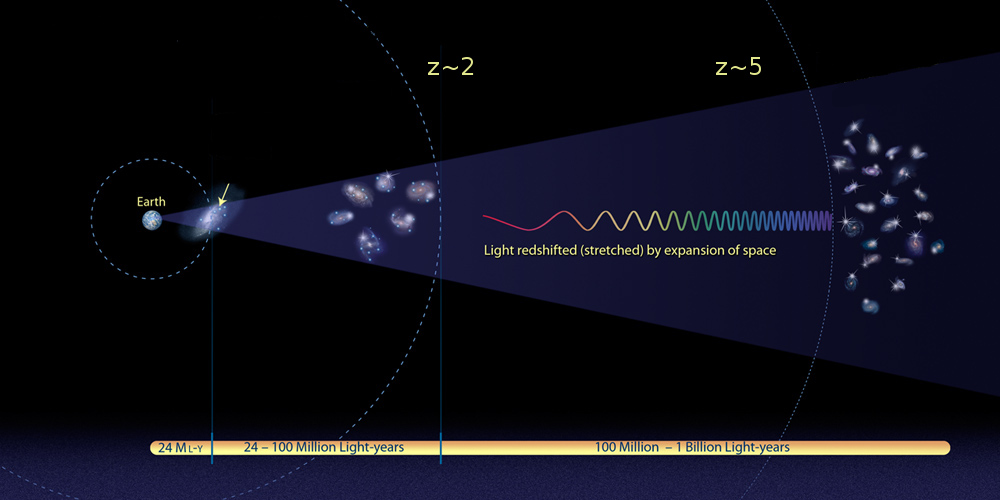
\includegraphics[scale=0.3]{Figures/expansion.jpg}
\caption{Image credit: NASA, ESA, and A. Feild (STScI).}
\end{figure}
\end{frame}

\begin{frame}
\begin{center}
\LARGE{Do galaxies radiate Ly$\alpha$ photons?}
\end{center}
\end{frame}

\begin{frame}{Hydrogen in the most abundant element in the Universe.} 
\begin{figure}
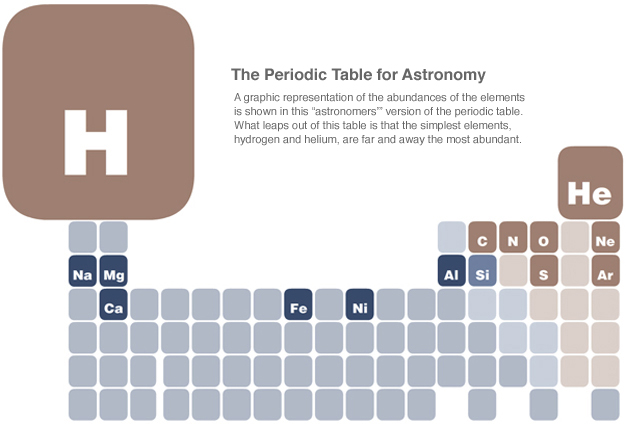
\includegraphics[scale=0.3]{Figures/astronomy_table.jpg}
\caption{Astronomers periodic table. Image credit: http://chandra.harvard.edu}
\end{figure}
\end{frame}

\begin{frame}{UV radiation mechanisms and sources:}

\begin{itemize}
\item UV stellar radiation 
\item Gravitational cooling
\item UV background radiation
\end{itemize}

\end{frame}

\begin{frame}%n{figure}
\begin{figure}
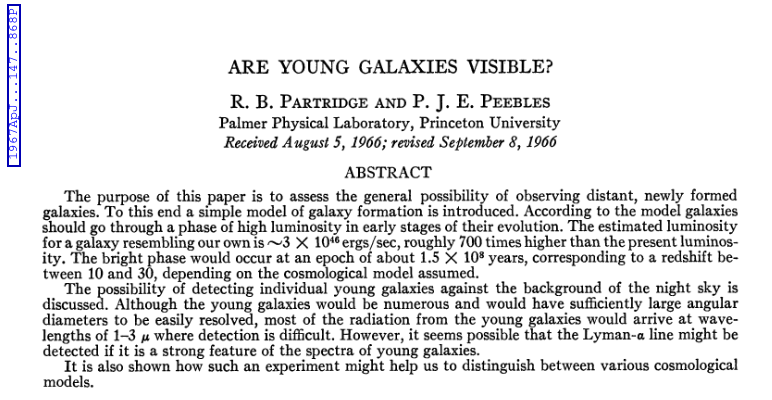
\includegraphics[scale=0.4]{Figures/PP.png}
\end{figure}
\end{frame}


\begin{frame}
\LARGE{25 years later ...}
\end{frame}

\begin{frame}
\begin{figure}
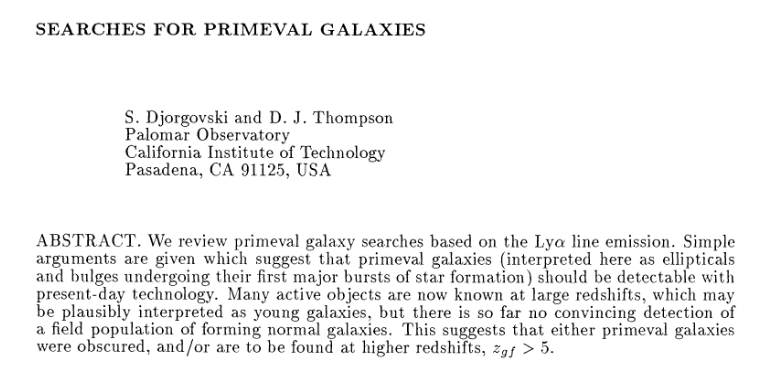
\includegraphics[scale=0.4]{Figures/DJT.png}
\end{figure}
\end{frame}

\begin{frame}{Ly $\alpha$ as an important tool in extragalactic astronomy}

\end{frame}

\begin{frame}{Units convention:}
\begin{equation}
V = \dfrac{\nu_{obs} - \nu_{\alpha}}{c}
\end{equation}
\end{frame}

\begin{frame}{LAEs spectra}
\begin{figure}
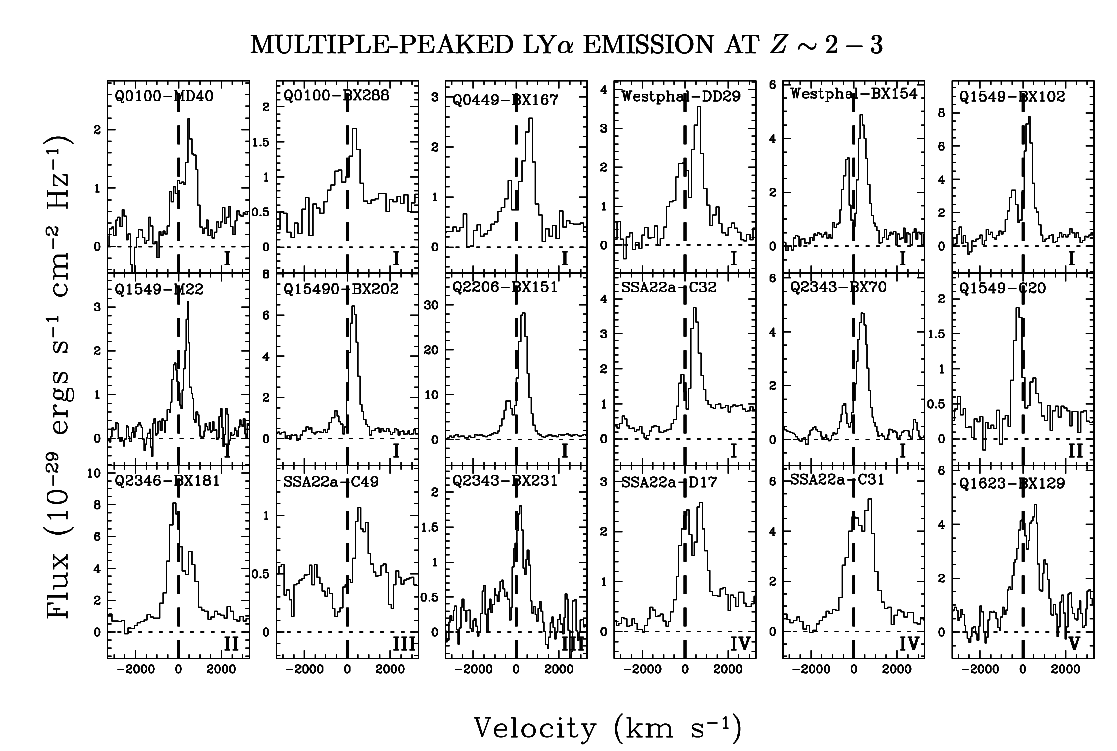
\includegraphics[scale=0.3]{Figures/kulas.png}
\end{figure}
\end{frame}

\begin{frame}{Radiative transfer through a static medium:}
\begin{figure}
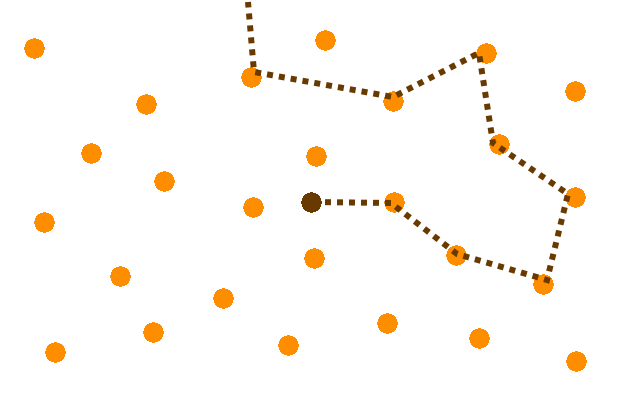
\includegraphics[scale=0.4]{Figures/RT.png}
\end{figure}
\end{frame}

\begin{frame}{Radiative transfer through a non-static medium:}
\begin{figure}
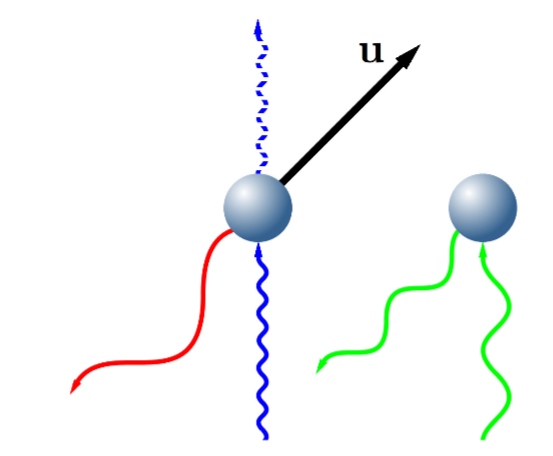
\includegraphics[scale=0.4]{Figures/xshift.png}
\end{figure}
\end{frame}


\begin{frame}{Ly$\alpha$ photons undergoes a random walk in space and wavelength}
\begin{figure}
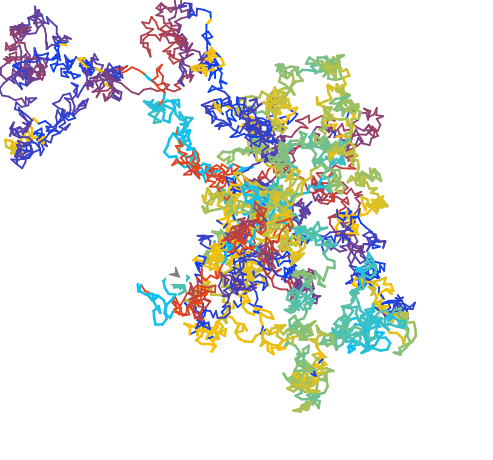
\includegraphics[scale=0.4]{Figures/rand_walk.png}
\end{figure}
\end{frame}

\begin{frame}{Dust and escape fraction of Ly$\alpha$ photons}

\end{frame}

\begin{frame}{Radiative transfer theory I:*}

\end{frame}

\begin{frame}{Radiative transfer theory II:*}

\end{frame}

%-------------------------- Previous studies ---------------------

\begin{frame}{Radiative Transfer via Monte-Carlo methods:}
\begin{itemize}
\item Set up the initial conditions (Temperature, gas distibution \& kinematics).
\item Set the Ly$\alpha$ photons initial positions $x_{in}$.
\item Generate the photon random displacement $\tau_0$ in a random direction
$\vec{n}$.
\item Derive the HI atom velocity components from the initial field and
generate random components for the thermal movements.
\item Set the new Ly$\alpha$ direction after the scattering.
\item Set the absorption probability due to dust encounters.
\item Iterate from step 2.
\end{itemize}
\end{frame}



\begin{frame}{Infinite slab:}
\begin{figure}
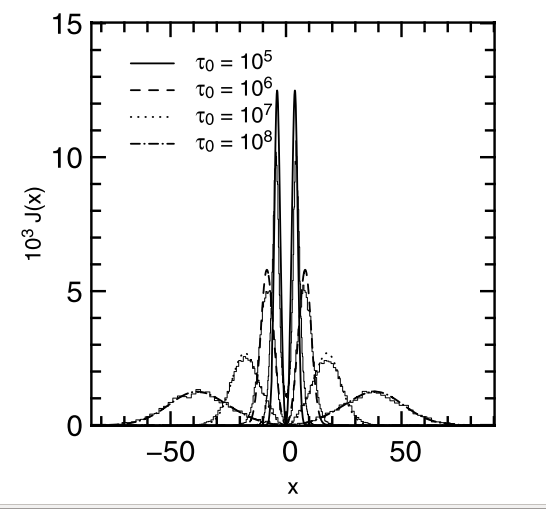
\includegraphics[scale=0.4]{Figures/slab.png}
\end{figure}
\end{frame}

\begin{frame}{Sphere with central sources:}
\begin{figure}
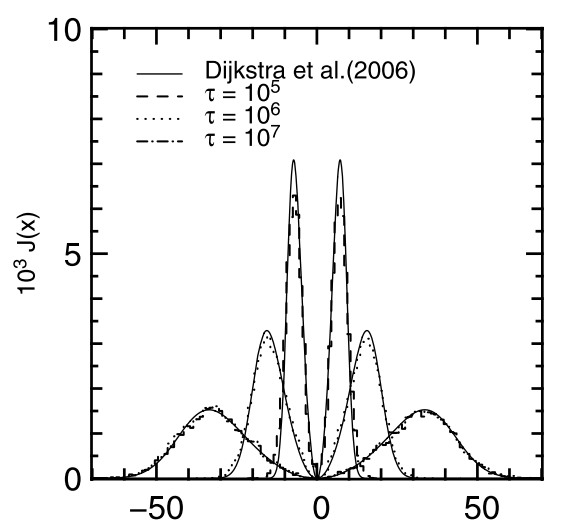
\includegraphics[scale=0.4]{Figures/sphere.png}
\end{figure}
\end{frame}

\begin{frame}{Sphere with homogeneous and central sources:}
\begin{figure}
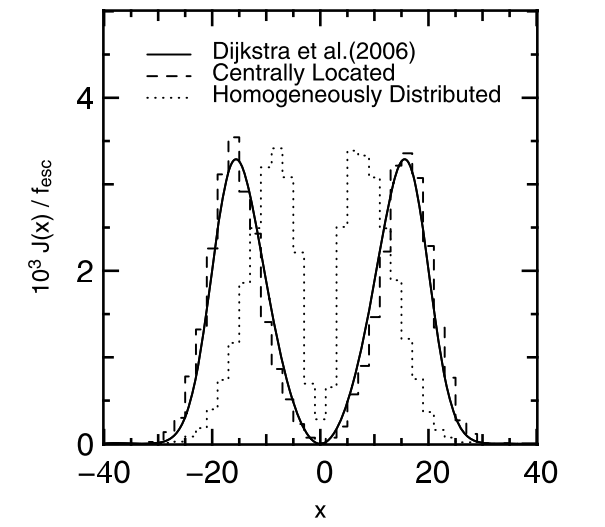
\includegraphics[scale=0.4]{Figures/homcen.png}
\end{figure}
\end{frame}

\begin{frame}
\LARGE{Different geometries have an impact on the morphology of the 
Ly$\alpha$ spectrum.}
\end{frame}

\begin{frame}{Expanding/Contracting sphere:}
\begin{figure}
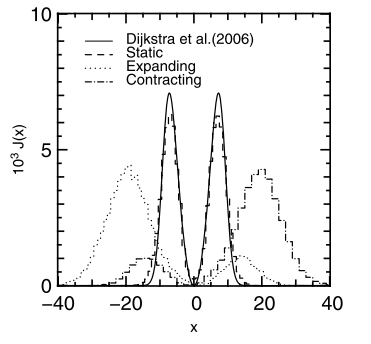
\includegraphics[scale=0.4]{Figures/expanding.png}
\end{figure}
\end{frame}

\begin{frame}{Cavities}
Zheng/Zheng and Dijkstra
\end{frame}

\begin{frame}{A SPH simulated galaxy spectrum}
\begin{figure}
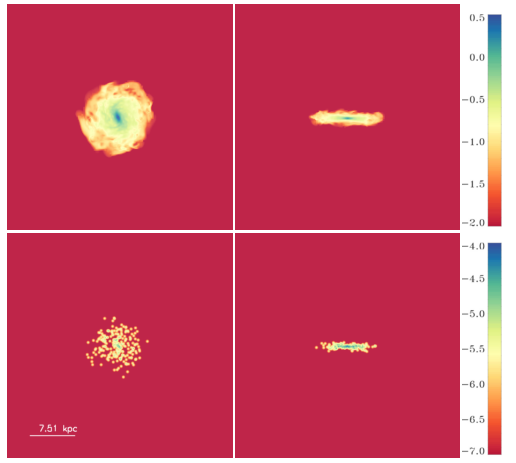
\includegraphics[scale=0.3]{Figures/verhamme1.png}
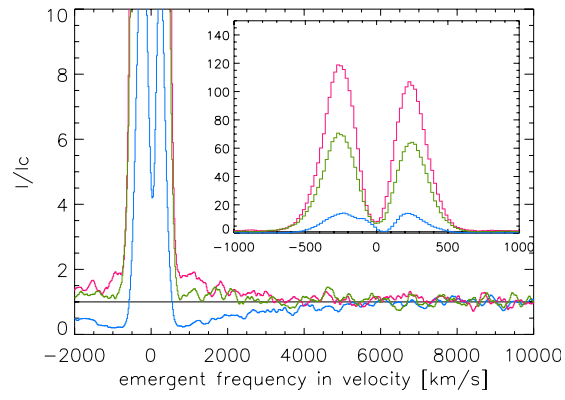
\includegraphics[scale=0.3]{Figures/Verhamme2.png}
\end{figure}
\end{frame}


%---------------------RESULTS-----------------------------

\begin{frame}
\begin{table}
\begin{center}
\begin{tabular}{llc}\hline\hline
Physical Parameter (units) & Symbol & Values\\\hline
Velocity ($km/s$) & $V_{\rm max}$&$0,\ \ 100,\ 200,\ 300$\\
Hydrogen Optical Depth & $\tau_{H} $ & $10^{5},\ 10^{6},\ 10^{7}$\\
Dust Optical Depth & $\tau_{a}$ & $0$,$1$\\
Photons Distributions & & Central, Homogeneous\\\hline\hline
\end{tabular}
\caption{Summary of Physical Parameters of our Monte Carlo Simulations.}
\end{center}
\end{table}
\end{frame}



\begin{frame}
\LARGE{We measure the impact of rotation and viewing angle $\theta$ in the 
main line characteristics characteristics}
\end{frame}

\begin{frame}{Simulated spectra}
\begin{figure}
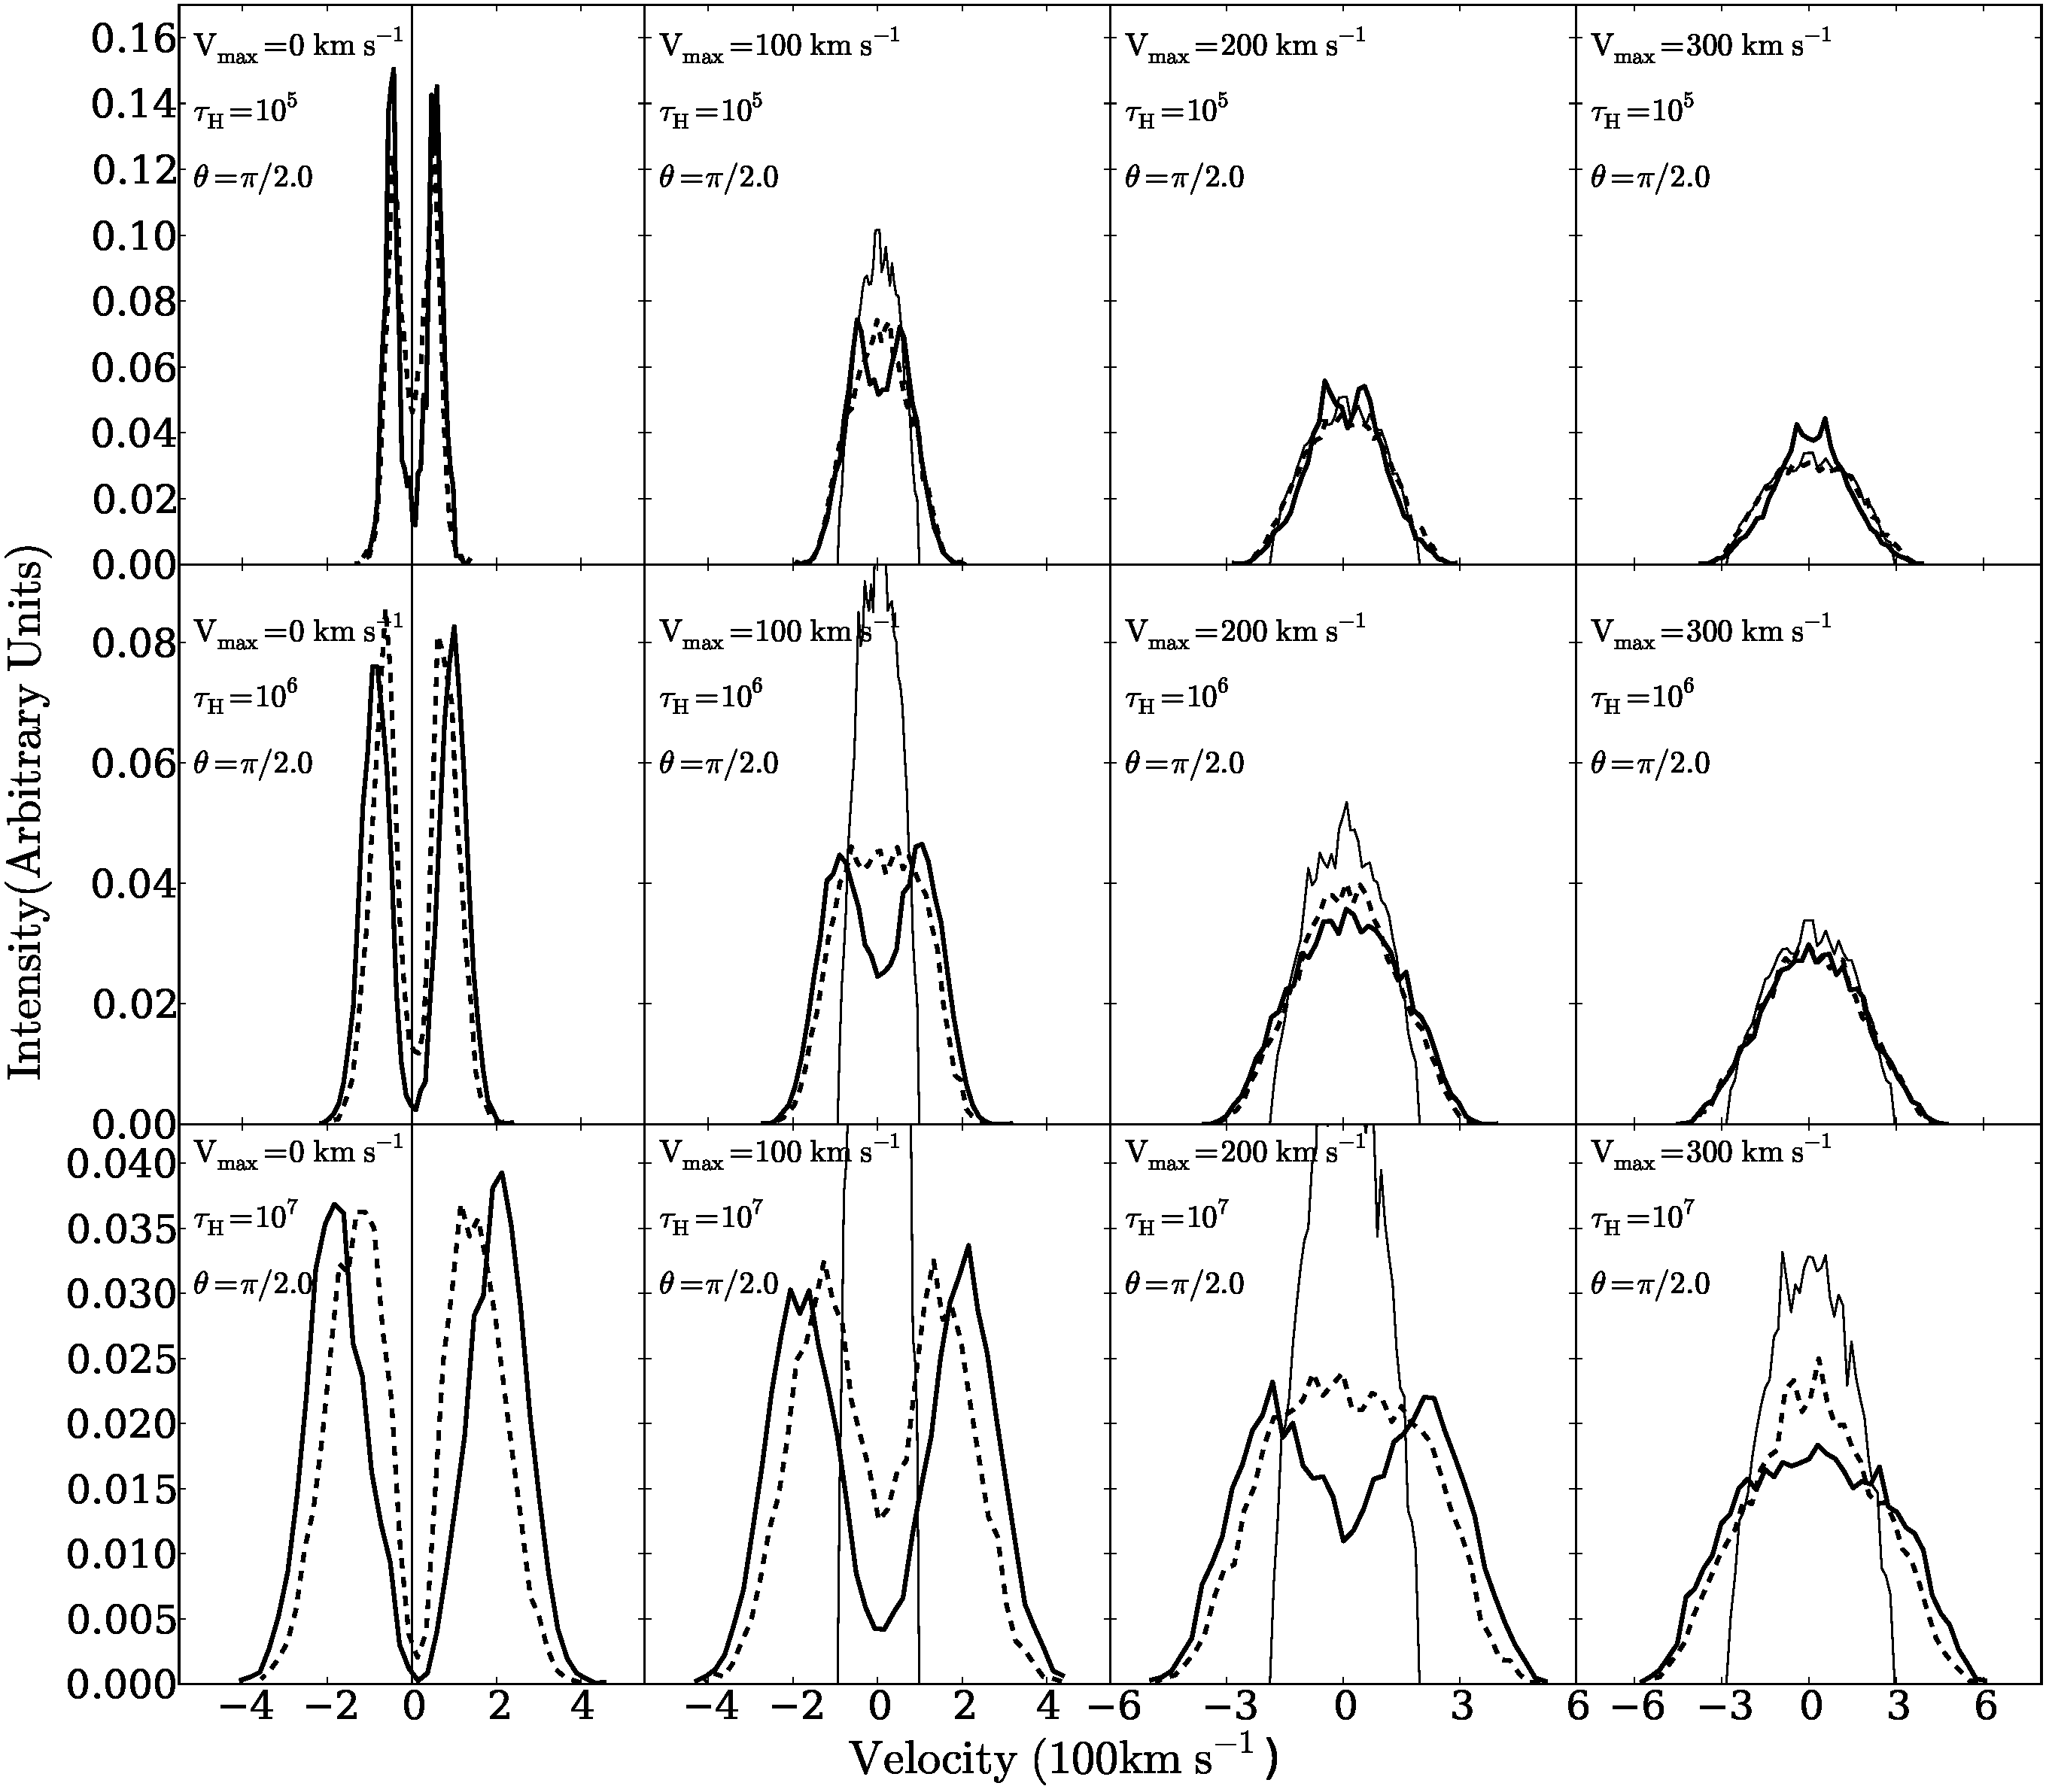
\includegraphics[scale=0.16]{Figures/f4.pdf}
\end{figure}
\end{frame}

\begin{frame}{Simulated spectra}
\begin{figure}
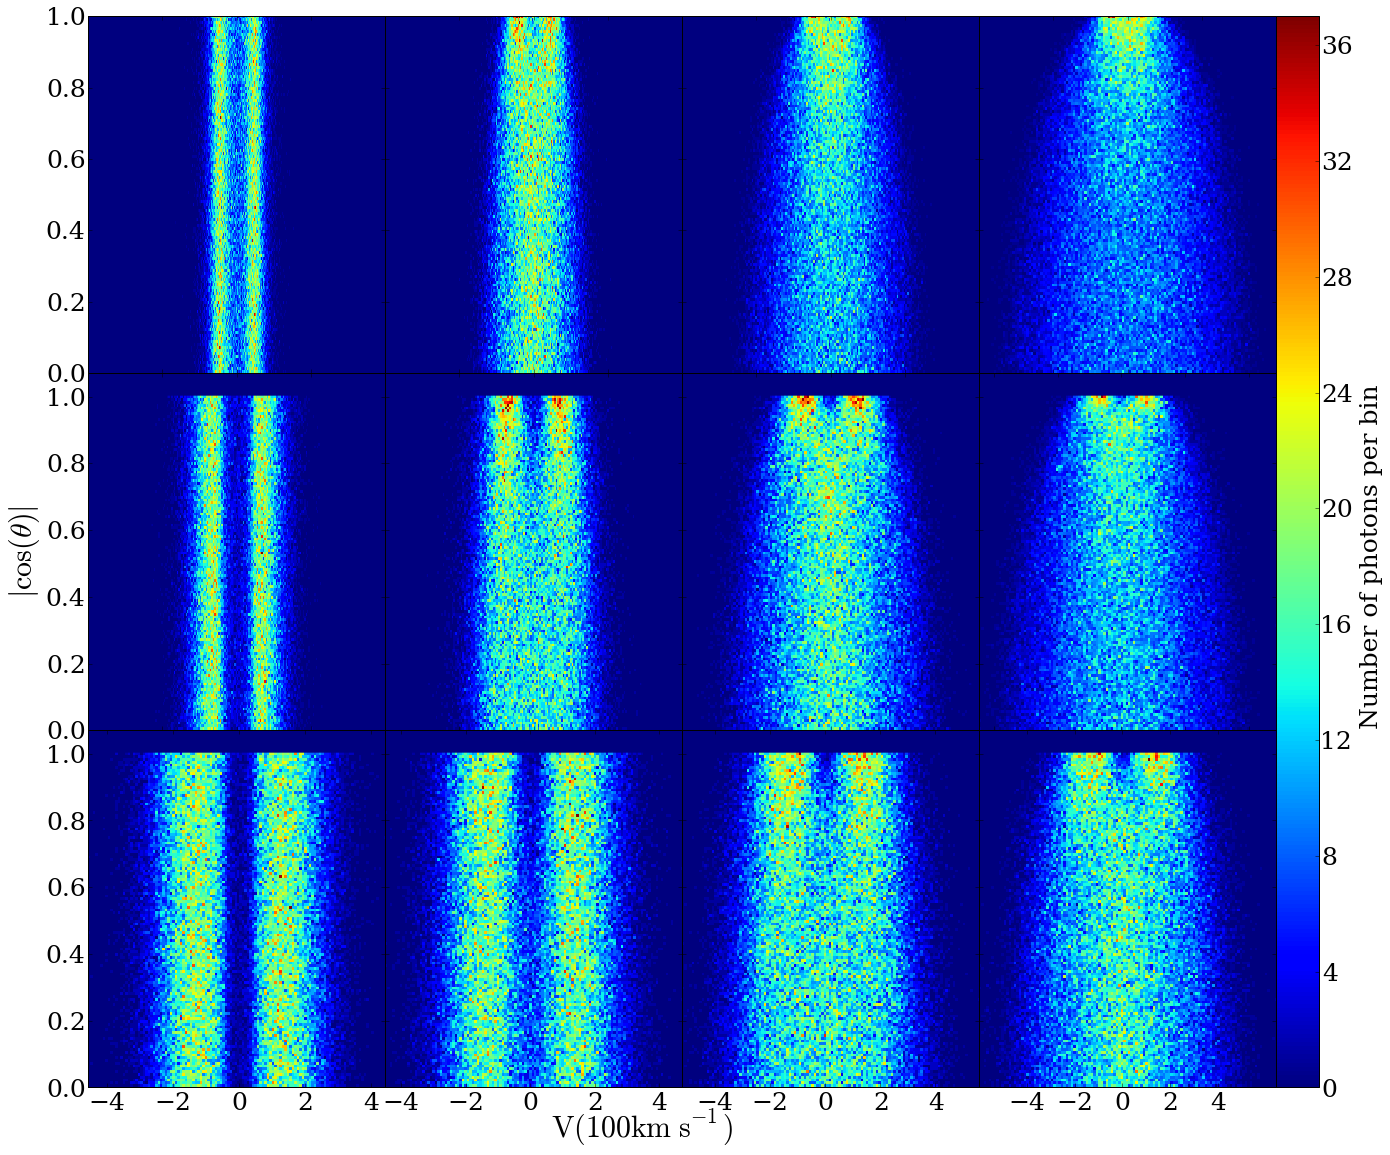
\includegraphics[scale=0.16]{Figures/f2.png}
\end{figure}
\end{frame}

\begin{frame}{Simulated spectra}
\begin{figure}
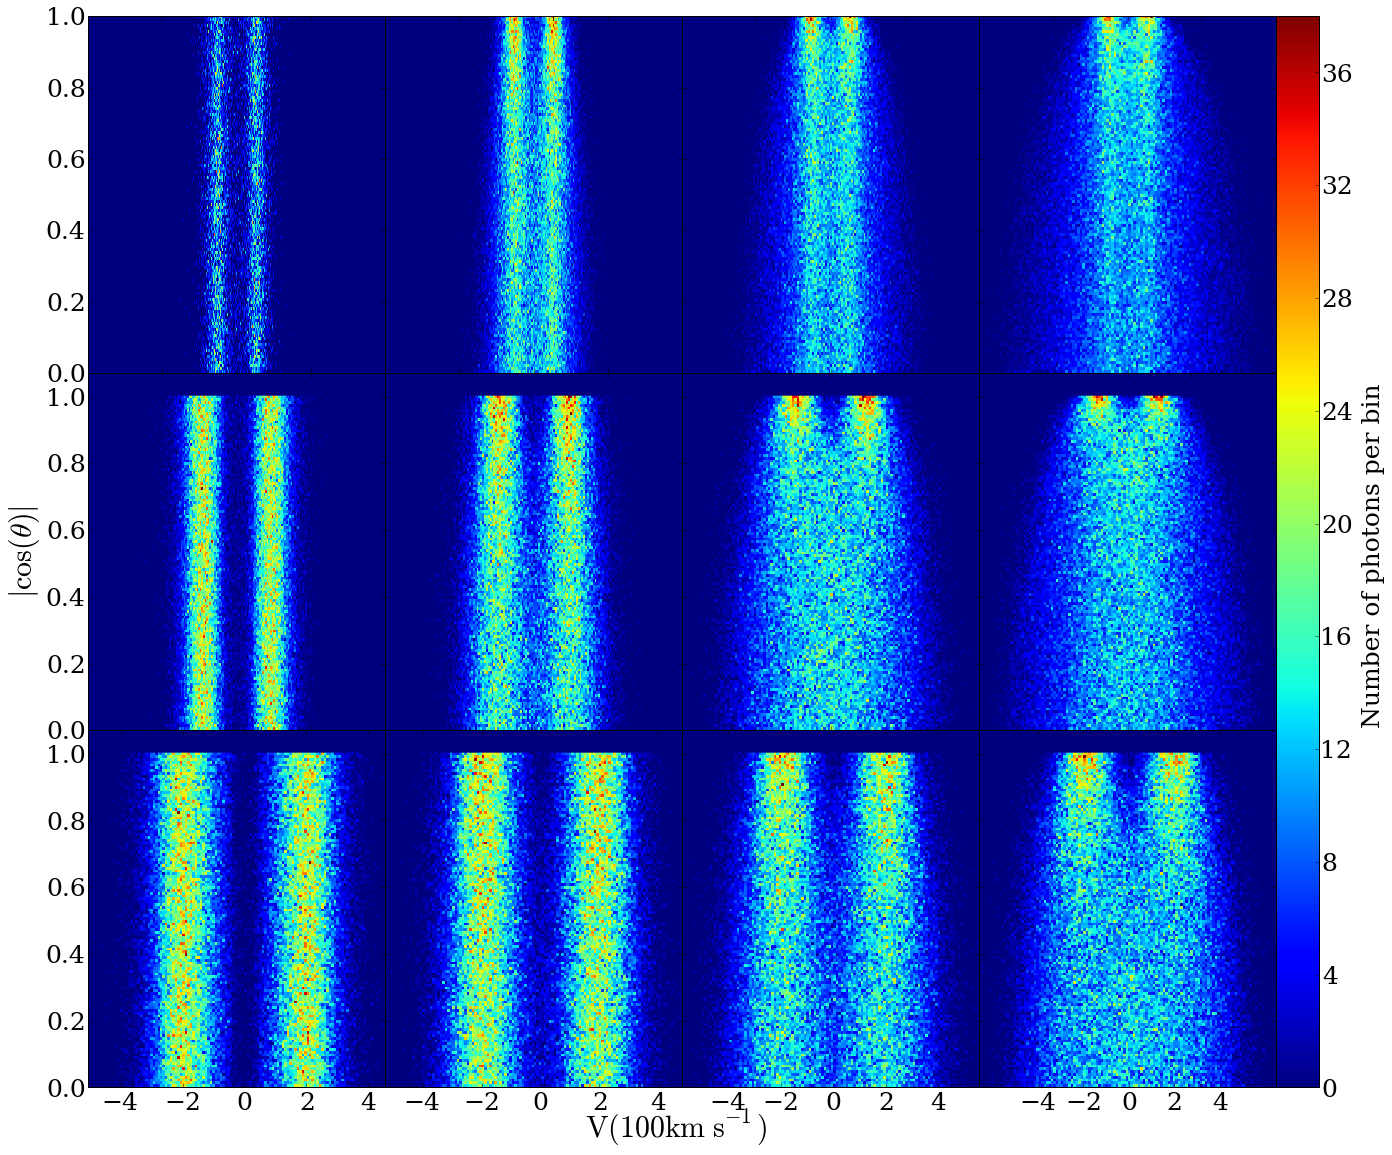
\includegraphics[scale=0.16]{Figures/f3.png}
\end{figure}
\end{frame}

\begin{frame}{Simulated spectra}
\begin{figure}
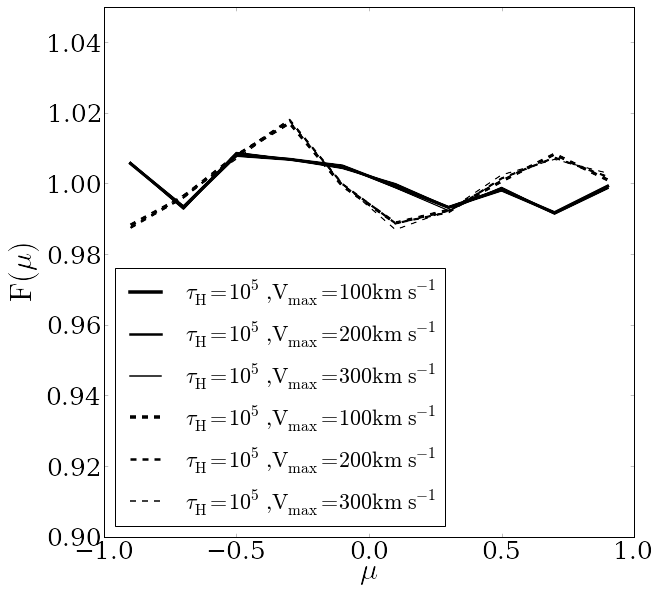
\includegraphics[scale=0.4]{Figures/f5.png}
\end{figure}
\end{frame}


\begin{frame}{The width of the line increases proportional with the rotation velocity.}
\begin{figure}
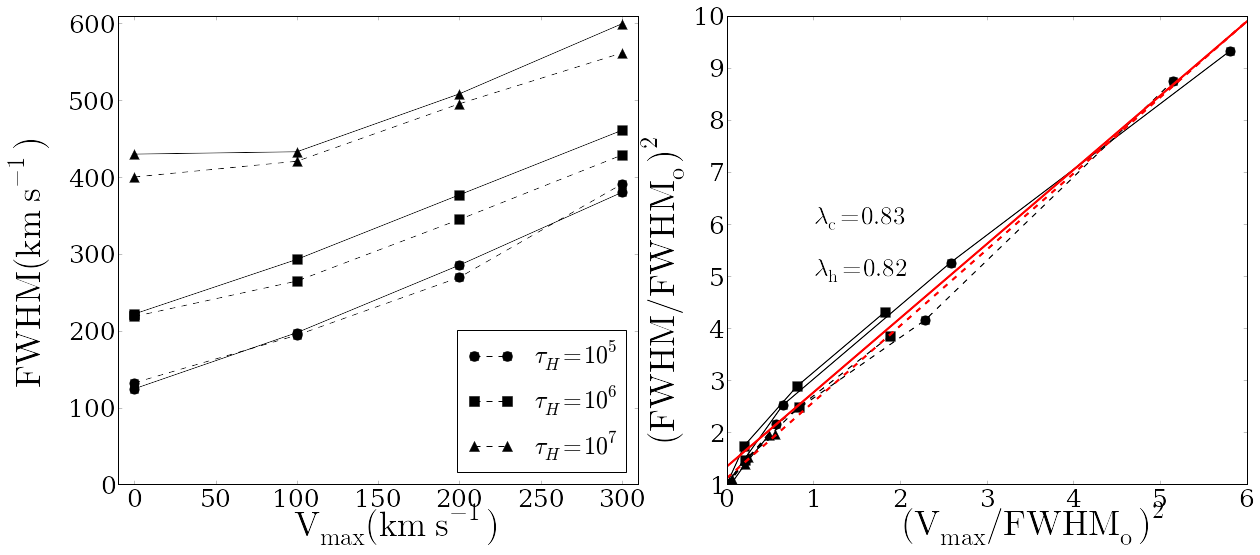
\includegraphics[scale=0.16]{Figures/f7.png}
\end{figure}
\end{frame}


\begin{frame}{The width of the line increases proportional with the rotation velocity.}
\begin{figure}
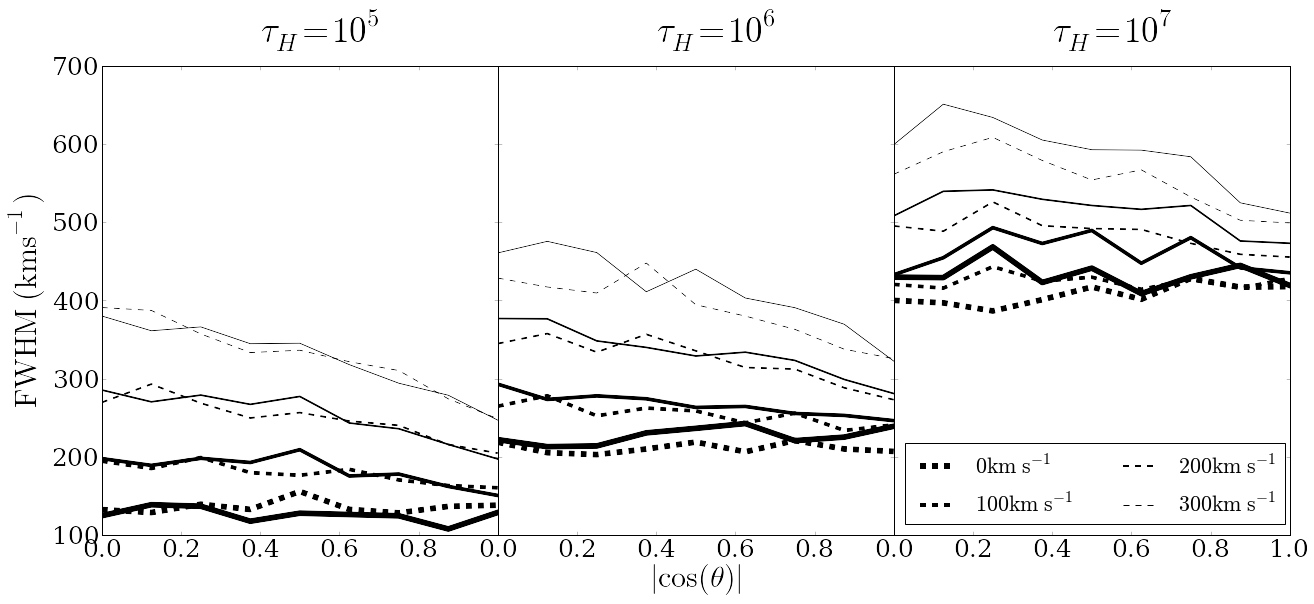
\includegraphics[scale=0.16]{Figures/f6.png}
\end{figure}
\end{frame}

\begin{frame}{The width of the line increases proportional with the rotation velocity.}
\begin{figure}
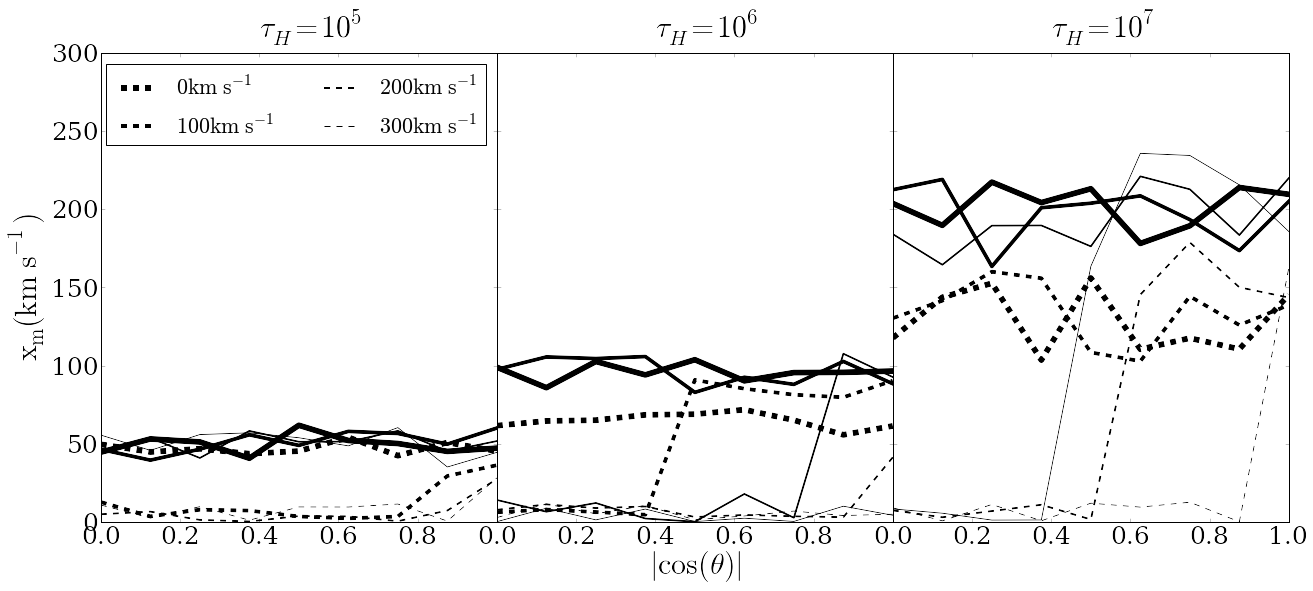
\includegraphics[scale=0.16]{Figures/f8.png}
\end{figure}
\end{frame}

\begin{frame}{The width of the line increases proportional with the rotation velocity.}
\begin{figure}
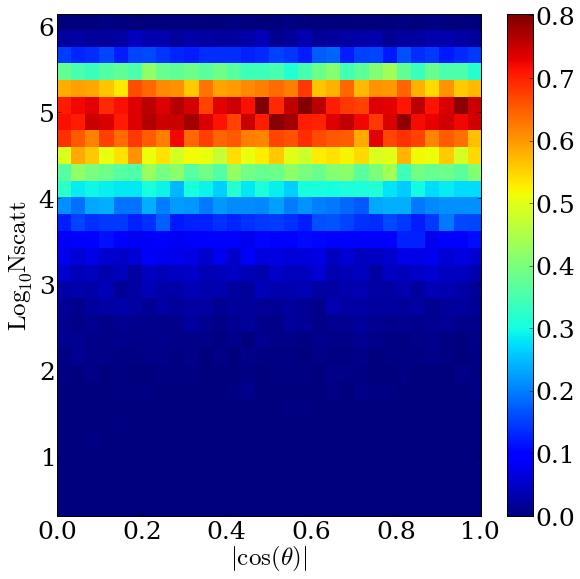
\includegraphics[scale=0.16]{Figures/f9h.png}
\end{figure}
\end{frame}

\begin{frame}{The width of the line increases proportional with the rotation velocity.}
\begin{figure}
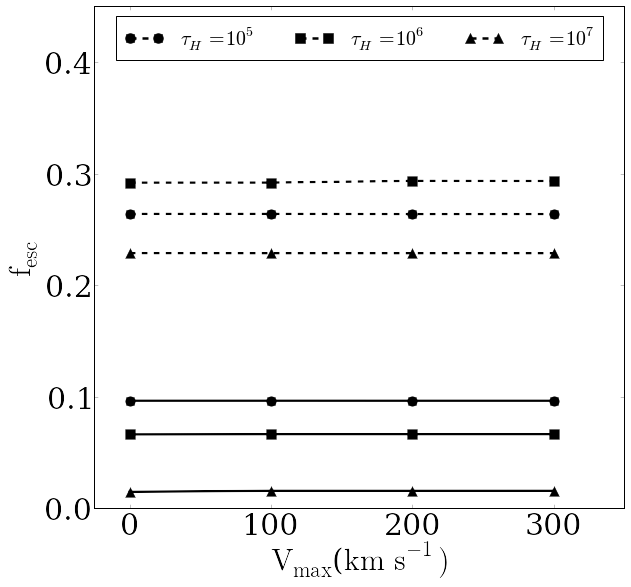
\includegraphics[scale=0.16]{Figures/f10.png}
\end{figure}
\end{frame}

\begin{frame}{Analytic aproximation}

\end{frame}

\begin{frame}{Analytic aproximation}

\end{frame}{Lyman alpha observed in rotation}

\begin{frame}

\end{frame}

\begin{frame}{Conclusions}
\end{frame}

\begin{frame}{Work in progress}
fit of the line
\end{frame}

\begin{frame}{Work in progress}
rotation + outfloes
\end{frame}

\end{document}
